\section{多元标量函数的一阶微分}
\label{sec:multivariable-scalar-first-order}

上一节回顾的极限与连续只问函数值是否趋近，本节开始度量函数值变化的快慢。最直接的办法是沿一条直线把多元函数变成一元函数，再求一元导数，这样得到偏导数和方向导数。

偏导数和方向导数只描述固定直线上的变化。接下来要判断，这些方向信息何时组成一个对全部小扰动都有效的线性近似，即全微分。全微分是作用于输入扰动的线性泛函；借助对偶空间与内积，它可以由输入空间中的一个向量表示，这个向量就是梯度。最后沿线段使用一元中值定理，把梯度的大小转化为有限变化的界。

本节研究实值函数$f:U\subseteq\mathbb R^d\to\mathbb R$，并要求$U$为开集。开集中每一点都有一个含于$U$的小球，从基点出发向任何方向走足够小的一步仍在定义域内，双侧差商因而都有意义。

\subsection{偏导数与方向导数}

固定除$x_j$以外的全部坐标，$f$就变成只依赖$x_j$的一元函数，它的导数就是偏导数。
\begin{definition}[偏导数]
\label{def:multivariable-partial-derivative}
设$\bm a\in U$，令$\bm e_j$是第$j$个坐标为$1$、其余为$0$的向量。若双侧极限
\[
 \partial_jf(\bm a)=\frac{\partial f}{\partial x_j}(\bm a)
 =\lim_{t\to0}\frac{f(\bm a+t\bm e_j)-f(\bm a)}t
\]
存在且有限，就称它为$f$在$\bm a$处关于$x_j$的\term{偏导数}（partial derivative）。
\end{definition}
偏导数是只改变第$j$个坐标、其余坐标固定时的变化率。符号$\partial$提醒我们，这里求的是一个坐标切片的导数。
对二元函数，$\partial_xf(a,b)$是用竖直平面$y=b$截曲面所得曲线在$x=a$处的切线斜率；$\partial_yf(a,b)$则来自平面$x=a$的截线。把$f$看成平板上的温度，$\partial_xf$就是向正东移动时温度每单位距离的变化。

计算偏导数时，把其余坐标当作常数，按一元函数求导即可。
\begin{example}[二次函数的偏导数]
\label{ex:multivariable-quadratic-partials}
对$f(x,y)=x^2+xy+y^2$，把$y$当作常数对$x$求导，得到$f_x=2x+y$；把$x$当作常数对$y$求导，得到$f_y=x+2y$。
在$(1,2)$处，两者分别为$4$和$5$。这种“把其余坐标当常数”的算法与定义一致，可以拿第一个值来验证：
\[
 \frac{f(1+t,2)-f(1,2)}t=\frac{(1+t)^2+2(1+t)+4-7}{t}=4+t\longrightarrow4.
\]
偏导数还能预测沿坐标方向走一小步时函数值的增量。$f(1.01,2)=7.0401$，比$f(1,2)=7$大约$0.04=4\times0.01$；$f(1,2.01)=7.0501$，大约大$5\times0.01$。两个预测都只差$10^{-4}$，即步长的平方。
\end{example}

$f_x(1,2)=4$并不意味着朝任何方向走都以斜率$4$变化，每个偏导数只描述自己那条坐标切片。若同时走$(0.01,0.01)$，则$f(1.01,2.01)=7.0903$，增量约为$0.04+0.05$，像是两个偏导数的贡献之和。这样相加并非总是成立；第~\ref{sec:multivariable-total-differentiation}节的可微性正是它成立的保证。

\paragraph{方向导数}

沿坐标轴求导只考察了$d$个方向。让多个坐标按一个固定向量的比例共同移动，就得到另一条直线上的一元切片，它的导数称为方向导数。
\begin{definition}[方向导数]
\label{def:multivariable-directional-derivative}
给定向量$\bm v\in\mathbb R^d$，若双侧极限
\[
 D_{\bm v}f(\bm a)
 =\lim_{t\to0}\frac{f(\bm a+t\bm v)-f(\bm a)}t
\]
存在且有限，就称它为沿$\bm v$的\term{方向导数}（directional derivative）。
\end{definition}
回到地形的比喻：站在$\bm a$上方，沿地图上的方向$\bm v$前进，方向导数就是脚下的坡度。
取$\bm v=\bm e_j$便回到偏导数。定义用的是双侧极限；只令$t\downarrow0$得到的单侧方向导数是另一个概念，存在与否要分别判断。若基点在定义域的边界上，例如闭区域的边界点，只有指向区域内部的方向才允许取小的正步长，这时只能讨论单侧差商，并须先说明哪些方向可以使用。本章只在开集内部使用双侧定义。

本书允许$\bm v$不是单位向量。这时导数按参数$t$计量：$t$增加$1$，水平位置移动$\lVert\bm v\rVert_2$。若要表示每单位水平距离的变化率，应取$\lVert\bm v\rVert_2=1$。比较同一条直线的两种参数化，就能看到方向向量的长度怎样改变方向导数的数值。
\begin{example}[沿对角方向的方向导数]
\label{ex:multivariable-diagonal-directional-derivative}
仍取$f(x,y)=x^2+xy+y^2$，从$(1,2)$沿$\bm v=(1,1)^\top$移动，展开得
\[
 f(1+t,2+t)=(1+t)^2+(1+t)(2+t)+(2+t)^2=7+9t+3t^2,
\]
所以$D_{\bm v}f(1,2)=9$。
改用同向单位向量$\bm u=(1,1)^\top/\sqrt2$，参数$t$增加$1$时只走过单位距离，变化率为$D_{\bm u}f(1,2)=9/\sqrt2\approx6.36$。
\end{example}

两个方向向量描述同一条直线，只是参数速度不同，所以比较变化率时要先统一归一化约定。
还可以注意到$9=4\cdot1+5\cdot1$：沿$(1,1)^\top$的变化率恰好是两个偏导数按方向分量加权之和。到这里我们只记录了一条条切片上的变化率。它们能否组成一个对所有方向、乃至方向不断改变的扰动都有效的线性近似，是下一小节要回答的问题。

\subsection{全微分与可微性判别}
\label{sec:multivariable-total-differentiation}

一元可微的含义是$f(a+h)=f(a)+f'(a)h+o(h)$：在$a$附近，函数图像可以用一条切线代替，误差比$h$小得多。把图像放大来看，曲线越来越像一条直线。
两个输入时，与切线对应的是切平面。把曲面$z=f(x,y)$在一点附近不断放大，如果它越来越像一张平面，就说$f$在该点可微；这张平面给出函数增量的线性近似。

预测增量的规则应与扰动的叠加和数乘相容，所以用线性映射$A:\mathbb R^d\to\mathbb R$来预测。
例如$A(\bm h)=\bm c^\top\bm h$把每个坐标的扰动乘以固定系数再相加。此外，预测遗漏的误差必须比扰动长度小得多。
\begin{definition}[多元标量函数的可微性与全微分]
\label{def:multivariable-total-differential}
设$U\subseteq\mathbb R^d$开，$f:U\to\mathbb R$，$\bm a\in U$。
若存在一个线性映射$A:\mathbb R^d\to\mathbb R$，使
\begin{equation}
\begin{gathered}
f(\bm a+\bm h)=f(\bm a)+A(\bm h)+o(\lVert\bm h\rVert_2)\\
\bm h\to\bm0,
\end{gathered}
\label{eq:analysis-total-differentiability}
\end{equation}
则称$f$在$\bm a$处\term{可微}（differentiable）。线性映射$A$称为该点的\term{全微分}（total differential），记为$\mathrm df_{\bm a}$。
\end{definition}
余项条件是
\[
 \frac{|f(\bm a+\bm h)-f(\bm a)-A(\bm h)|}{\lVert\bm h\rVert_2}\longrightarrow0,
\]
其中$\bm h\to\bm 0$按第~\ref{sec:multivariable-joint-limits}节的联合极限理解。
它要求同一个$A$适用于全部趋零扰动，而不是先固定一个方向、再按方向分别控制误差。
$d=2$时，$z=f(\bm a)+A(\bm x-\bm a)$是三维空间中经过$(\bm a,f(\bm a))$的一张平面，即切平面。余项条件说的是：曲面与切平面的高度差比到$\bm a$的水平距离小得多。

用数值可以看到这个“小得多”。
\begin{example}[切平面误差随步长缩小]
\label{ex:multivariable-tangent-plane-error}
仍看$f(x,y)=x^2+xy+y^2$在$(1,2)$处，用线性映射$A(h,k)=4h+5k$预测增量（示例~\ref{ex:multivariable-quadratic-differential}将证明它就是全微分），并观察误差相对步长怎样变化。
沿$(h,k)=(0.01,0.02)$走一步，切平面预测$7+0.04+0.10=7.14$，实际值$f(1.01,2.02)=7.1407$，误差为$0.0007$，与步长$\sqrt{0.01^2+0.02^2}\approx0.0224$之比约为$0.031$。
把步长减半为$(0.005,0.01)$，误差缩小到$0.000175$，只有原来的四分之一；它与步长$\approx0.0112$之比约为$0.016$，恰好减半。
\end{example}

误差与步长之比随步长减半而减半；步长继续缩小时，这个比值趋于零，这正是余项条件的要求。

\paragraph{可微性的要求与判别}
\label{sec:analysis-differentiability-relations}

以下固定开集$U\subseteq\mathbb R^d$、标量函数$f:U\to\mathbb R$与基点$\bm a\in U$。
先看可微必然带来什么，再给出一个便于核查的充分条件，最后用反例区分偏导数存在、全部双侧方向导数存在、可微和连续可微。

\paragraph{可微的必要条件}
若同一个线性近似对全部扰动有效，把扰动限制在一条直线上，它就必须与这条直线上的一元导数相同；函数增量本身也必须趋于零。
由这两点可以把全微分与偏导数及方向导数联系起来。
\begin{theorem}[可微性与偏导数、方向导数]
\label{thm:multivariable-differentiable-necessary}
若$f:U\to\mathbb R$在$\bm a$处可微，则$f$在该点连续，各偏导数存在，全微分唯一，并且
\[
 \begin{gathered}
\mathrm df_{\bm a}(\bm h)=\sum_{j=1}^d\partial_jf(\bm a)h_j\\
D_{\bm v}f(\bm a)=\mathrm df_{\bm a}(\bm v)
 \quad(\bm v\in\mathbb R^d).
 \end{gathered}
\]
\end{theorem}
\begin{proof}
记$A=\mathrm df_{\bm a}$。先证连续。把$\bm h$按标准基写成$\sum_jh_j\bm e_j$，线性性给出$A(\bm h)=\sum_jh_jA(\bm e_j)$。由有限和的Cauchy--Schwarz不等式，
\[
 |A(\bm h)|\leq\left(\sum_j|A(\bm e_j)|^2\right)^{1/2}\lVert\bm h\rVert_2,
\]
这也就是第~\ref{sec:multivariable-operator-norm}节所说的有限维线性映射的Lipschitz连续性。因此在式~\eqref{eq:analysis-total-differentiability}中，线性项与余项都随$\bm h\to\bm 0$而趋零，即$f(\bm a+\bm h)\to f(\bm a)$，$f$连续。

再求系数。取$\bm h=t\bm e_j$，式~\eqref{eq:analysis-total-differentiability}变成$f(\bm a+t\bm e_j)-f(\bm a)=tA(\bm e_j)+o(|t|)$；两边除以$t$并令$t\to0$，可知偏导数存在且$\partial_jf(\bm a)=A(\bm e_j)$。代回线性展开，得到$A(\bm h)=\sum_j\partial_jf(\bm a)h_j$。任何满足式~\eqref{eq:analysis-total-differentiability}的线性映射在每个$\bm e_j$上的值都由同一个偏导数确定，所以全微分唯一。
最后对固定的$\bm v\neq\bm0$取$\bm h=t\bm v$：差商等于$A(\bm v)$加上余项除以$t$，而余项是$o(|t|\lVert\bm v\rVert_2)$，除以$t$后仍趋零，就得到方向导数公式；$\bm v=\bm0$时差商恒为零。
\end{proof}
定理说明，一旦可微，全微分只能是以各偏导数为系数的线性映射，所有方向导数也都由这$d$个偏导数线性地决定。
因此验证可微时，候选线性映射已经确定，只需再估计余项。对本章的二次函数，这一步可以直接完成。
\begin{example}[二元二次函数的全微分]
\label{ex:multivariable-quadratic-differential}
对二次函数$f(x,y)=x^2+xy+y^2$，在$(1,2)$处两个偏导数为$4$与$5$，候选线性映射为$(h,k)\mapsto4h+5k$。

设扰动为$(h,k)$，直接展开得
\[
 f(1+h,2+k)=7+4h+5k+(h^2+hk+k^2).
\]
由$|hk|\leq(h^2+k^2)/2$，最后一项绝对值不超过$3(h^2+k^2)/2$；除以$\sqrt{h^2+k^2}$后不超过$\tfrac32\sqrt{h^2+k^2}$，随扰动趋于零。所以全微分确为$\mathrm df_{(1,2)}(h,k)=4h+5k$，切平面为$z=7+4(x-1)+5(y-2)$。
\end{example}

这个全微分同时给出了示例~\ref{ex:multivariable-quadratic-partials}中的两个偏导数，以及示例~\ref{ex:multivariable-diagonal-directional-derivative}中沿$(1,1)^\top$的变化率$4+5=9$。
图~\ref{fig:analysis-process-total-differential-remainder}画出了这个切平面，以及对所有方向同时成立的余项界。
\begin{figure*}[!htbp]
 \centering
 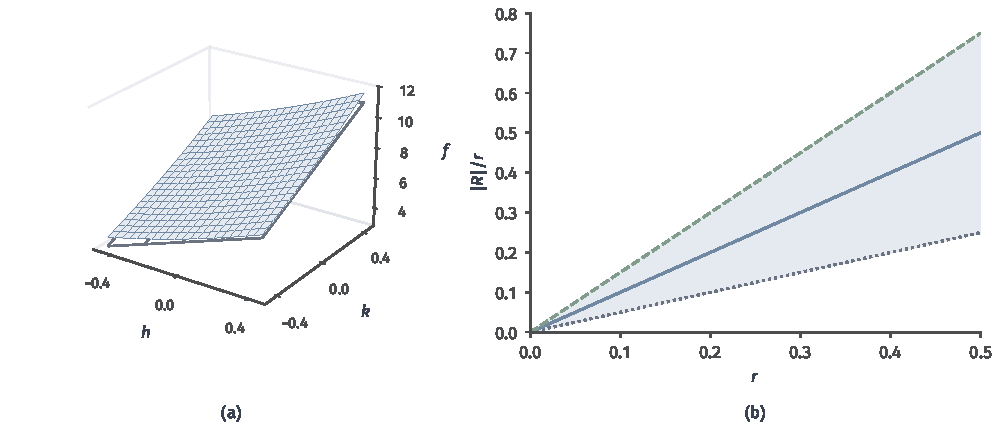
\includegraphics[width=169.0mm]{figures/00-shared/mathematical-preliminaries-upper/00-shared/matplotlib/chapter3-concept-processes/total-differential-remainder.pdf}
 \caption{(a) 二次函数在$(1,2)$附近，灰网格是切平面$P=7+4h+5k$，蓝面是$f(1+h,2+k)$。(b) 令$r=\sqrt{h^2+k^2}$，余项$R=h^2+hk+k^2$满足$r/2\leq R/r\leq3r/2$；阴影给出所有方向的完整范围，三条线是其中的代表值。共同上界随$r\to0$趋零，才保证任意方向都适用同一个线性近似。}
 \label{fig:analysis-process-total-differential-remainder}
\end{figure*}

\paragraph{偏导数连续给出的充分条件}
按定义验证可微需要估计余项，通常不方便。另一种判别只检查偏导数：如果各坐标的变化率在基点附近连续变化，就可以沿坐标逐段走，用它们共同控制全部坐标增量。
与定理~\ref{thm:multivariable-differentiable-necessary}不同，这是一个充分条件，直接保证全微分存在。
\begin{theorem}[偏导数连续与可微性]
\label{thm:multivariable-continuous-partials-sufficient}
设$f:U\to\mathbb R$，$U$开，$\bm a\in U$。若各一阶偏导数在$\bm a$的某个邻域内存在，并在$\bm a$处连续，则$f$在$\bm a$处可微。
\end{theorem}
\begin{proof}
先看$d=2$。从$(a_1,a_2)$走到$(a_1+h_1,a_2+h_2)$，可以先竖直走、再水平走：
\[
 \begin{aligned}
 &f(a_1+h_1,a_2+h_2)-f(a_1,a_2)\\
 &=\bigl[f(a_1+h_1,a_2+h_2)-f(a_1,a_2+h_2)\bigr]\\
 &\quad+\bigl[f(a_1,a_2+h_2)-f(a_1,a_2)\bigr].
 \end{aligned}
\]
第一个方括号只改变第一个坐标，对一元函数$s\mapsto f(s,a_2+h_2)$用中值定理，得到它等于$\partial_1f(\bm\xi_1)h_1$，其中$\bm\xi_1$在这段水平线段上；第二个方括号同理等于$\partial_2f(\bm\xi_2)h_2$，$\bm\xi_2$在竖直线段上。这里用到$\bm h$足够小时两段都在偏导数存在的邻域内。

一般的$d$同样把$\bm a$到$\bm a+\bm h$的增量拆成$d$段，每段只改一个坐标，一元中值定理将第$j$段增量写成$\partial_jf(\bm\xi_j)h_j$，$\bm\xi_j$是第$j$段上的中间点。
减去候选线性项后，误差为$\sum_j\bigl(\partial_jf(\bm\xi_j)-\partial_jf(\bm a)\bigr)h_j$，因此
\[
 \begin{aligned}
 &\left|f(\bm a+\bm h)-f(\bm a)-\sum_{j=1}^d\partial_j f(\bm a)h_j\right|\\
 &\qquad\leq \max_j\left|\partial_j f(\bm\xi_j)-\partial_j f(\bm a)\right|
       \sum_{j=1}^d|h_j|
 =o(\lVert\bm h\rVert_2).
 \end{aligned}
\]
最后一步有两个依据：当$\bm h\to\bm0$时，所有中间点到$\bm a$的距离都不超过$\lVert\bm h\rVert_2$，偏导数在$\bm a$处连续，使最大值一项趋于零；另一方面$\sum_j|h_j|\leq\sqrt d\lVert\bm h\rVert_2$。
这样，各坐标方向上的变化就拼成了同一个有效的全微分。
\end{proof}
偏导数连续只是充分条件：可微只要求函数增量有统一的一阶近似，不要求这些系数随基点连续变化。实际计算中，若各偏导数在所论开集上由连续的表达式给出，就可以直接断定可微。多项式、分母非零的有理函数，以及它们与指数、正弦等连续函数的复合，都属于这种情形。

\paragraph{连续可微函数}
若要求全微分的系数在一个范围内随基点连续变化，就得到连续可微的概念。
实值函数的各一阶偏导数在开集$U$上存在且连续时，称它在$U$上连续可微，记为$C^1(U)$；$C^k(U)$表示直至$k$阶的各偏导数都存在且连续。
定理~\ref{thm:multivariable-continuous-partials-sufficient}保证$C^1$函数处处可微。逆向并不成立，一元函数就足以说明这一点。
\begin{example}[处处可微而导数无界]
\label{ex:multivariable-differentiable-not-c1}
在实轴上令$r(0)=0$，$x\neq0$时令$r(x)=x^2\sin(1/x^2)$。
由于$|r(h)/h|=|h\sin(1/h^2)|\leq|h|\to0$，有$r'(0)=0$；非零点按运算法则求导，得到
\[
 r'(x)=2x\sin(1/x^2)-\frac{2}{x}\cos(1/x^2).
\]
取$x_n=(2\pi n)^{-1/2}$，则$1/x_n^2=2\pi n$，$\sin$项为$0$、$\cos$项为$1$，于是$r'(x_n)=-2/x_n\to-\infty$。所以$r$处处可微，$r'$却在$0$附近无界，在$0$处不连续。
直观上，$r$的振幅被$x^2$压到零，图像在原点与横轴相切；但振荡越来越快，切线斜率剧烈摆动。
在多元情形令$f(\bm x)=r(x_1)$，就得到处处可微而非连续可微的标量函数。
\end{example}

这个例子还说明可微不保证局部Lipschitz连续（定义~\ref{def:ls-lipschitz}）。若$r$在原点的某个邻域内以$L$为Lipschitz常数，该邻域内每个差商的绝对值都不超过$L$，各点导数也就满足$|r'|\leq L$，与$r'(x_n)\to-\infty$矛盾。

\paragraph{必要条件不能反推可微}
可微蕴含连续、偏导数存在和全部双侧方向导数存在。一元函数在一点的导数存在就等价于可微，因为实轴上只有一条直线可走。多元函数还须协调无穷多个输入方向以及弯曲的趋近路径，所以这些必要条件单独或合起来都不能保证可微。下面依次检查它们的逆向。

\paragraph{偏导数存在不保证可微}
坐标偏导数只约束两条坐标切片，并未控制其余方向或路径。
\begin{example}[偏导数存在但不可微]
\label{ex:analysis-partials-not-differentiable}
定义$f:\mathbb{R}^2\to\mathbb{R}$为
\[
 f(x,y)=
 \begin{cases}
  \dfrac{xy}{\sqrt{x^2+y^2}}, & (x,y)\neq(0,0),\\[6pt]
  0, & (x,y)=(0,0).
 \end{cases}
\]
沿两条坐标轴，函数恒为$0$，所以$\partial f/\partial x(0,0)=\partial f/\partial y(0,0)=0$。若$f$在原点可微，由定理~\ref{thm:multivariable-differentiable-necessary}，候选线性部分只能是零映射。可是沿$\bm{h}=(t,t)$，
\[
 \frac{|f(t,t)-f(0,0)|}{\lVert(t,t)\rVert_2}
 =\frac{|t|/\sqrt{2}}{\sqrt{2}|t|}
 =\frac12,
\]
余项与$\lVert\bm{h}\rVert_2$之比不趋于零，故$f$在原点不可微。

用极坐标可以看清曲面的形状：$f=r\cos\theta\sin\theta=\tfrac r2\sin2\theta$。沿每条从原点出发的射线，函数随$r$线性增长，斜率$\tfrac12\sin2\theta$随方向变化。曲面由这些射线组成，像一个起伏的锥面；把它放大任意倍数后形状不变，永远不会变得像一张平面。

沿每个方向$\bm v=(a,b)$，只令$t\downarrow0$的正向方向导数都存在，等于$ab/\sqrt{a^2+b^2}$（零方向取$0$），但它不是关于$\bm v$的线性函数。$t<0$时差商变号，因此$ab\neq0$时双侧方向导数不存在。
最后，由$|xy|/\sqrt{x^2+y^2}\leq\sqrt{x^2+y^2}/2$，$f$在原点连续。
\end{example}

偏导数只看坐标轴，遗漏了其他接近方向；可微则要求曲面放大后接近平面，本例的锥面做不到。本例还说明，即使偏导数存在、全部正向方向导数存在、函数又连续，也推不出可微。这里的正向方向导数是单侧极限，与本节采用的双侧定义不同，使用时要分清。

\paragraph{全部方向导数存在不保证可微}
把坐标切片换成所有固定直线，仍有两件事需要检查：这些变化率能否组成一个线性映射，以及是否有统一的余项控制。先看缺少线性性的情形。
\begin{example}[方向导数不构成线性映射]
\label{ex:multivariable-nonlinear-directional-derivatives}
在非原点处令$p(x,y)=x^3/(x^2+y^2)$，并令$p(0,0)=0$。
沿$\bm v=(a,b)\neq\bm0$，差商为$p(ta,tb)/t=a^3/(a^2+b^2)$，不依赖$t$，所以双侧方向导数存在且$D_{\bm v}p(0,0)=a^3/(a^2+b^2)$。
取坐标方向得到两个偏导数$1$与$0$。若$p$可微，由定理~\ref{thm:multivariable-differentiable-necessary}，沿$(1,1)^\top$的方向导数应为$1\cdot1+0\cdot1=1$，实际却是$1/(1+1)=1/2$。这些方向变化率无法拼成一个线性映射，所以$p$在原点不可微。
\end{example}

示例~\ref{ex:analysis-partials-not-differentiable}只有单侧方向导数；这里的双侧方向导数全部存在，失败只来自线性性。
即使方向导数全部存在并组成一个线性映射，还要检查余项能否统一控制。
\begin{example}[方向导数全为零仍不可微]
\label{ex:multivariable-linear-directionals-not-differentiable}
在非原点处令$q(x,y)=x^3y/(x^4+y^2)$，并令$q(0,0)=0$。
由$2|x^2y|\leq x^4+y^2$，有$|q(x,y)|\leq|x|/2$，故$q$在原点连续。
对固定方向$(a,b)^\top$，若$b\neq0$，
\[
 \frac{q(ta,tb)}t=\frac{t a^3b}{t^2a^4+b^2}\longrightarrow0;
\]
若$b=0$，差商恒为零。因此所有双侧方向导数都为零，它们组成零线性映射。
可是沿$\bm h=(t,t^2)^\top$，$q(t,t^2)=t^5/(2t^4)=t/2$，从而
\[
 \frac{|q(t,t^2)|}{\lVert(t,t^2)\rVert_2}
 =\frac1{2\sqrt{1+t^2}}\longrightarrow\frac12.
\]
候选零映射不满足全微分的余项条件，$q$在原点不可微。
\end{example}

这与示例~\ref{ex:multivariable-parabola-path-limit}中$g$的情形相同：函数沿抛物线有一道坡，每条直线进入原点时都避开了它。方向导数先固定方向再取极限；全微分则要求方向随扰动改变时，误差仍受同一个控制。

\paragraph{连续与偏导数存在互不蕴含}
连续性也推不出微分条件。
例如$f(x,y)=|x|$在整个平面上Lipschitz连续，图像沿$y$轴有一道折痕。原点关于$x$的双侧偏导数不存在，因此$f$在那里不可微。
偏导数存在同样推不出连续：示例~\ref{ex:multivariable-path-limits}中原点置零的$xy/(x^2+y^2)$沿坐标轴恒为零，两个偏导数存在，但它在原点不连续。
所以连续与偏导数存在互不蕴含，可微则同时保证二者。

\paragraph{条件之间的蕴含关系}
把必要条件、充分判别与上面的反例放在一起，得到下面的蕴含链：
\[
 \begin{gathered}
 f\text{在}\bm a\text{的某邻域内连续可微}
 \ \Longrightarrow\ f\text{在}\bm a\text{处可微},\\
 f\text{在}\bm a\text{处可微}
 \ \Longrightarrow\ \text{全部双侧方向导数存在}
 \ \Longrightarrow\ \text{全部偏导数存在}.
 \end{gathered}
\]
第一条由定理~\ref{thm:multivariable-continuous-partials-sufficient}得到，第二条由定理~\ref{thm:multivariable-differentiable-necessary}得到，最后一条只须在全部方向中取坐标方向$\bm e_j$。
同一定理还说明，可微蕴含连续，并且方向导数关于方向是线性映射$\bm v\mapsto\mathrm df_{\bm a}(\bm v)$。
第一行的前提涉及$\bm a$的整个邻域，其余条件只涉及基点$\bm a$本身；链中的方向导数都按双侧极限理解。

各箭头都不能反向：示例~\ref{ex:multivariable-differentiable-not-c1}说明处处可微仍可能不连续可微；示例~\ref{ex:multivariable-nonlinear-directional-derivatives}与示例~\ref{ex:multivariable-linear-directionals-not-differentiable}说明全部双侧方向导数存在仍可能不可微，后者连函数连续、方向导数组成线性映射这两点也都满足；示例~\ref{ex:analysis-partials-not-differentiable}说明偏导数存在不推出全部双侧方向导数存在。不满足偏导数连续这一充分条件时，应回到全微分的定义检查余项。

\subsection{微分的运算法则}
\label{sec:multivariable-differential-rules}

直接按定义求全微分很繁琐。与一元情形一样，可以从简单函数的微分出发，用运算法则组合出复杂函数的微分。
本小节的$f,g$都在同一开集内定义，并在基点$\bm a$处可微，$c$为固定实数。
各法则的证明方法相同：代入各自的一阶展开，整理出关于$\bm h$的线性项，再确认剩下的部分仍是$o(\lVert\bm h\rVert_2)$。这样既证明新函数可微，也读出了它的全微分。

\paragraph{和、差与数乘的微分}
把两个一阶展开相加，
\[
 (f+g)(\bm a+\bm h)=(f+g)(\bm a)+\bigl(\mathrm df_{\bm a}+\mathrm dg_{\bm a}\bigr)(\bm h)+o(\lVert\bm h\rVert_2),
\]
两个线性映射之和仍是线性映射，两个$o(\lVert\bm h\rVert_2)$余项之和仍是$o(\lVert\bm h\rVert_2)$，因此
$\mathrm d(f+g)=\mathrm df+\mathrm dg$。
把加号换成减号，同样的论证给出$\mathrm d(f-g)=\mathrm df-\mathrm dg$。固定系数$c$只会缩放线性项与余项，故$\mathrm d(cf)=c\,\mathrm df$，包括$c=0$的常函数情形。

\paragraph{积的微分}
记$R_f,R_g$为两个一阶展开的余项，都是$o(\lVert\bm h\rVert_2)$。相乘得
\[
 \begin{aligned}
 f(\bm a+\bm h)g(\bm a+\bm h)
 &=\bigl(f(\bm a)+\mathrm df(\bm h)+R_f\bigr)\bigl(g(\bm a)+\mathrm dg(\bm h)+R_g\bigr)\\
 &=f(\bm a)g(\bm a)+g(\bm a)\,\mathrm df(\bm h)+f(\bm a)\,\mathrm dg(\bm h)+(\text{其余各项}).
 \end{aligned}
\]
其余各项要么含有余项$R_f,R_g$乘以有界量，要么是两个线性增量的乘积$\mathrm df(\bm h)\,\mathrm dg(\bm h)=O(\lVert\bm h\rVert_2^2)$，都是$o(\lVert\bm h\rVert_2)$。因此乘积可微，且
\[
 \mathrm d(fg)=g(\bm a)\,\mathrm df+f(\bm a)\,\mathrm dg.
\]
这与一元的$(fg)'=f'g+fg'$形式相同：两个因子各自变化，一阶上贡献可以相加，两个变化同时发生的部分是高阶小量。

\paragraph{商的微分}
设$g(\bm a)\neq0$。可微蕴含连续，所以$g$在$\bm a$附近远离零，$1/g$在$\bm a$附近有定义。记$\delta=g(\bm a+\bm h)-g(\bm a)=\mathrm dg(\bm h)+o(\lVert\bm h\rVert_2)$，它是$O(\lVert\bm h\rVert_2)$。一元函数$1/y$在$g(\bm a)$处的展开给出
\[
 \frac1{g(\bm a)+\delta}=\frac1{g(\bm a)}-\frac{\delta}{g(\bm a)^2}+O(\delta^2).
\]
代入$\delta$的展开，并注意$O(\delta^2)=O(\lVert\bm h\rVert_2^2)$，得到$\mathrm d(1/g)=-\mathrm dg/g(\bm a)^2$。再把$f/g$看成$f\cdot(1/g)$，用积的微分得到
\[
 \mathrm d(f/g)=\frac{g(\bm a)\,\mathrm df-f(\bm a)\,\mathrm dg}{g(\bm a)^2}.
\]
这里分母非零既是定义商函数的条件，也是估计余项的条件。

\paragraph{标量复合函数的微分}
若一元函数$\psi$在$f(\bm a)$处可微，且复合在$\bm a$的邻域内有定义，则$\psi\circ f$在$\bm a$处可微，并且
\[
 \mathrm d(\psi\circ f)=\psi'(f(\bm a))\,\mathrm df.
\]
推导时把内层增量$\delta=f(\bm a+\bm h)-f(\bm a)$代入外层的一元展开$\psi(f(\bm a)+\delta)=\psi(f(\bm a))+\psi'(f(\bm a))\delta+o(|\delta|)$，再把$\delta=\mathrm df(\bm h)+o(\lVert\bm h\rVert_2)$代入。
因为$\delta=O(\lVert\bm h\rVert_2)$，外层余项$o(|\delta|)$仍是$o(\lVert\bm h\rVert_2)$。
例如$-(x^2+y^2)$在$(x,y)$处的全微分为$(h,k)\mapsto-2xh-2yk$，所以$e^{-(x^2+y^2)}$的全微分是$(h,k)\mapsto e^{-(x^2+y^2)}(-2xh-2yk)$：外层只把内层的全微分乘上一个正数。

\paragraph{沿参数曲线的变化率}
外层也可以是多元函数、内层是一元的参数曲线。设$\bm x:I\to U$定义在开区间$I$上，各坐标在$t_0$处可微，记速度向量$\bm x'(t_0)=(x_1'(t_0),\ldots,x_d'(t_0))^\top$；又设$f$在$\bm a=\bm x(t_0)$处可微。则$t\mapsto f(\bm x(t))$在$t_0$处可微，且
\begin{equation}
 \frac{\mathrm d}{\mathrm dt}f(\bm x(t))\Big|_{t=t_0}
 =\mathrm df_{\bm a}\bigl(\bm x'(t_0)\bigr)
 =\sum_{j=1}^d\partial_jf(\bm a)\,x_j'(t_0).
\label{eq:multivariable-curve-chain-rule}
\end{equation}
推导与上一段相同。记内层增量$\bm k=\bm x(t_0+s)-\bm x(t_0)$，各坐标的一元展开给出$\bm k=s\bm x'(t_0)+o(|s|)$，因而$\lVert\bm k\rVert_2=O(|s|)$。代入$f$的一阶展开，
\[
 f(\bm x(t_0+s))-f(\bm a)=\mathrm df_{\bm a}(\bm k)+o(\lVert\bm k\rVert_2)
 =s\,\mathrm df_{\bm a}(\bm x'(t_0))+o(|s|),
\]
第二步用了全微分的线性，以及线性映射把长度为$o(|s|)$的向量仍变成$o(|s|)$的数。除以$s$并令$s\to0$即得。
内层的变化先在输入空间中产生速度向量$\bm x'(t_0)$，外层的全微分再作用于这个方向。取直线$\bm x(t)=\bm a+t\bm v$，便回到方向导数公式$D_{\bm v}f(\bm a)=\mathrm df_{\bm a}(\bm v)$。下一小节用式~\eqref{eq:multivariable-curve-chain-rule}说明梯度与等值曲线的切向正交；一般向量值映射的复合在第~\ref{sec:analysis-vector-chain-matrix-calculus}节处理。

\paragraph{二次型的微分}
二次型是向量自变量的标量函数，平方误差、能量函数等都含有这种结构。考虑$q(\bm{x})=\bm{x}^{\top}\bm{A}\bm{x}=\sum_{i,j}A_{i,j}x_ix_j$，其中$\bm{A}\in\mathbb{R}^{d\times d}$固定。它是有限个乘积的和，可以直接用乘积法则：把两个$\bm x$看成两个因子，每次只让一个变化，
\begin{align*}
  \mathrm{d}q_{\bm x}(\bm h)
  &=
  \bm h^{\top}\bm{A}\bm{x}
  +\bm{x}^{\top}\bm{A}\bm h\\
  &=
  \bm{x}^{\top}(\bm{A}^{\top}+\bm{A})\bm h.
\end{align*}
第二步用到$\bm h^\top\bm A\bm x$是一个实数，等于自己的转置$\bm x^\top\bm A^\top\bm h$。所以全微分的系数，即各偏导数排成的列向量，为
\begin{equation}
  \bigl(\partial_1q(\bm x),\ldots,\partial_dq(\bm x)\bigr)^\top
  =
  (\bm{A}+\bm{A}^{\top})\bm{x}.
\label{eq:analysis-quadratic-form-gradient}
\end{equation}
当$\bm{A}$对称时，式~\eqref{eq:analysis-quadratic-form-gradient}化为$2\bm{A}\bm{x}$，与一元的$(ax^2)'=2ax$对应。$\bm A$不对称时不能写成$2\bm{A}\bm{x}$，否则就默认了对称性。
例如
\[
 \bm A=\begin{bmatrix}0&1\\0&0\end{bmatrix}
\]
时$q=x_1x_2$，直接求偏导得$(x_2,x_1)^\top$，与$(\bm A+\bm A^\top)\bm x$一致；而$2\bm A\bm x=(2x_2,0)^\top$是错的。

\paragraph{二次型的精确增量}
乘积法则只给出一阶项。对二次型还可以直接写出完整增量，把一阶项与实际误差放在同一个式子里。设$\bm S$对称，展开得
\[
 q(\bm x+\bm h)-q(\bm x)
 =\bm h^\top\bm S\bm x+\bm x^\top\bm S\bm h+\bm h^\top\bm S\bm h
 =2\bm x^\top\bm S\bm h+\bm h^\top\bm S\bm h,
\]
其中用到$\bm h^\top\bm S\bm x=(\bm h^\top\bm S\bm x)^\top=\bm x^\top\bm S\bm h$。由Cauchy--Schwarz不等式与谱范数的定义（第~\ref{sec:multivariable-operator-norm}节），
\[
 |\bm h^\top\bm S\bm h|\leq\lVert\bm h\rVert_2\lVert\bm S\bm h\rVert_2\leq\lVert\bm S\rVert_2\lVert\bm h\rVert_2^2 .
\]
所以余项不只是$o(\lVert\bm h\rVert_2)$，而是被一个明确的二次量控制；这也独立地证明了$q$可微，且$\mathrm dq_{\bm x}(\bm h)=2\bm x^\top\bm S\bm h$。
例如$x^2+xy+y^2=\bm x^\top\bm S\bm x$，其中
\[
 \bm S=\begin{bmatrix}1&1/2\\1/2&1\end{bmatrix}
\]
的特征值为$3/2$与$1/2$。对称矩阵的谱范数是特征值绝对值的最大者（第~\ref{chap:eigen-spectral-decomposition}章），故$\lVert\bm S\rVert_2=3/2$，这正是示例~\ref{ex:multivariable-quadratic-differential}中余项上界$\tfrac32(h^2+k^2)$的常数。
二次项$\bm h^\top\bm S\bm h$在第~\ref{sec:multivariable-curvature-error}节成为Hessian二次型，梯度和余项估计也将复用这个例子。

\subsection{梯度与内积}
\label{sec:multivariable-gradient-inner-product}

可微时，全微分$\mathrm df_{\bm a}$是$\mathbb R^d$上的线性泛函，即对偶空间中的元素（第~\ref{sec:ls-dual-spaces}节）：它读取一个输入扰动，给出函数值的一阶变化。泛函本身不是输入空间中的向量，不能画成地图上的箭头。第~\ref{sec:ls-riesz-representation}节的Riesz表示定理说明，选定内积后，每个线性泛函都等于与唯一一个向量的内积。把这个向量作为全微分的表示，就得到梯度。
\begin{definition}[梯度]
\label{def:multivariable-gradient}
设$\mathbb R^d$上取定内积$\langle\cdot,\cdot\rangle$，$f:U\to\mathbb R$在$\bm a$处可微。满足
\[
 \mathrm df_{\bm a}(\bm h)=\langle\nabla f(\bm a),\bm h\rangle\qquad(\bm h\in\mathbb R^d)
\]
的唯一向量$\nabla f(\bm a)\in\mathbb R^d$称为$f$在$\bm a$处的\term{梯度}（gradient）。未加说明时取标准欧氏内积$\langle\bm x,\bm y\rangle=\bm x^\top\bm y$。
\end{definition}
在标准欧氏内积下，比较定理~\ref{thm:multivariable-differentiable-necessary}中的$\mathrm df_{\bm a}(\bm h)=\sum_j\partial_jf(\bm a)h_j$与$\nabla f(\bm a)^\top\bm h$，逐个取$\bm h=\bm e_j$，得到
\begin{equation}
 \nabla f(\bm a)=\bigl(\partial_1f(\bm a),\ldots,\partial_df(\bm a)\bigr)^\top .
\label{eq:multivariable-gradient-coordinates}
\end{equation}
于是可微函数满足$f(\bm a+\bm h)=f(\bm a)+\nabla f(\bm a)^\top\bm h+o(\lVert\bm h\rVert_2)$，方向导数为$D_{\bm v}f(\bm a)=\nabla f(\bm a)^\top\bm v$。
例如$f(x,y)=x^2+xy+y^2$的梯度为$\nabla f(x,y)=(2x+y,x+2y)^\top$，$\nabla f(1,2)=(4,5)^\top$；由式~\eqref{eq:analysis-quadratic-form-gradient}，一般二次型有$\nabla_{\bm x}(\bm x^\top\bm A\bm x)=(\bm A+\bm A^\top)\bm x$。
梯度与输入属于同一个空间：$(4,5)^\top$可以画成地图平面上从$(1,2)$出发的一支箭头，而不是曲面上的向量。

若$f$在开集$U$上处处可微，把每一点的梯度放在该点，就得到$U$上的向量场$\nabla f:U\to\mathbb R^d$，称为$f$的梯度场。例如第~\ref{sec:multivariable-scalar-fields}节的标量场$x^2+y^2$的梯度场是$(2x,2y)^\top$，箭头从原点向外，离原点越远越长，与那里观察到的“等值圆越来越密”相符。哪些向量场是某个标量场的梯度场，留到第~\ref{sec:multivariable-potential-path-independence}节研究。

表示向量随泛函线性变化，所以上一小节的法则直接改写为梯度的法则：$\nabla(f\pm g)=\nabla f\pm\nabla g$，$\nabla(cf)=c\nabla f$，$\nabla(fg)=g(\bm a)\nabla f+f(\bm a)\nabla g$，$\nabla(\psi\circ f)=\psi'(f(\bm a))\nabla f$。例如$\nabla e^{-(x^2+y^2)}=e^{-(x^2+y^2)}(-2x,-2y)^\top$，与$-(x^2+y^2)$的梯度同向，都指向原点。

\paragraph{偏导数向量与梯度}
式~\eqref{eq:multivariable-gradient-coordinates}的右侧在偏导数全部存在时就能写出，本书在这种情形下也用记号$\nabla f(\bm a)$表示这一列偏导数。但第~\ref{sec:multivariable-total-differentiation}节的反例说明，这时它只是坐标变化率排成的向量：示例~\ref{ex:multivariable-nonlinear-directional-derivatives}中这一列是$(1,0)^\top$，却给不出沿$(1,1)^\top$的方向导数。只有确认可微以后，它才代表对所有方向同时有效的一阶近似，才可以用内积计算任意方向导数，并解释为最快上升的方向。

梯度的列向量排列也来自所选内积和坐标：全微分本身是一个线性作用，标准欧氏内积把它的系数原样排成列向量。换用其他内积时，同一个全微分由另一个向量表示。

\paragraph{改变内积时的梯度}
设$\mathbb R^d$上的内积在标准坐标下写成$\langle\bm x,\bm y\rangle_{\bm G}=\bm x^\top\bm G\bm y$，其中$\bm G$对称正定。第~\ref{sec:ls-gram-coordinates}节说明，任何内积在坐标下都是这种形式，$\bm G$就是基的Gram矩阵。记全微分的系数向量为$\bm c=\bigl(\partial_jf(\bm a)\bigr)_{j=1}^d$。要求$\mathrm df_{\bm a}(\bm h)=\bm c^\top\bm h=\bm g^\top\bm G\bm h$对所有$\bm h$成立，等价于$\bm G\bm g=\bm c$，所以
\begin{equation}
 \nabla_{\bm G}f(\bm a)=\bm G^{-1}\bigl(\partial_jf(\bm a)\bigr)_{j=1}^d .
\label{eq:multivariable-gradient-gram}
\end{equation}
系数向量$\bm c$由函数本身决定；改变的只是用哪个向量来表示同一个全微分。
\begin{example}[加权内积下的梯度]
\label{ex:multivariable-weighted-gradient}
仍取$f(x,y)=x^2+xy+y^2$与基点$(1,2)$，系数向量为$(4,5)^\top$。改用$\bm G=\operatorname{diag}(4,1)$给出的加权内积$\langle\bm x,\bm y\rangle_{\bm G}=4x_1y_1+x_2y_2$，由式~\eqref{eq:multivariable-gradient-gram}，
\[
 \nabla_{\bm G}f(1,2)=\operatorname{diag}(1/4,1)\,(4,5)^\top=(1,5)^\top.
\]
核对：$\langle(1,5)^\top,(h,k)^\top\rangle_{\bm G}=4h+5k$，正是同一个全微分。欧氏梯度$(4,5)^\top$与加权梯度$(1,5)^\top$方向不同：加权长度把第一坐标的位移计为原来的两倍，沿它走同样的加权距离只需更小的坐标位移。
\end{example}
这与第~\ref{sec:ls-riesz-representation}节的结论一致：读取本身不变，表示向量随内积改变。

\paragraph{最陡上升方向}
设$f$在$\bm a$处可微，$\bm u$满足$\lVert\bm u\rVert=1$，这里的长度由所选内积诱导。由Cauchy--Schwarz不等式（定理~\ref{thm:linear-algebra-cauchy-schwarz}），
\[
 D_{\bm u}f(\bm a)=\langle\nabla f(\bm a),\bm u\rangle\leq\lVert\nabla f(\bm a)\rVert.
\]
梯度非零时，取$\bm u=\nabla f(\bm a)/\lVert\nabla f(\bm a)\rVert$即达到等号。所以在所选内积的单位长度约束下，梯度方向是局部上升最快的方向，最大坡度等于梯度的长度；反方向$-\nabla f(\bm a)$则下降最快。
示例~\ref{ex:multivariable-weighted-gradient}中，欧氏单位长度下最快方向沿$(4,5)^\top$，加权单位长度下则沿$(1,5)^\top$。“最快”总是相对某种长度而言的。

\paragraph{梯度与等值曲线}
若$\bm u$与梯度正交，方向导数为零，函数值一阶上不变。设$\bm x:I\to U$是一条落在等值集$\{\bm y:f(\bm y)=f(\bm a)\}$中的可微曲线，$\bm x(t_0)=\bm a$。$f(\bm x(t))$恒为常数，由式~\eqref{eq:multivariable-curve-chain-rule}，
\[
 0=\frac{\mathrm d}{\mathrm dt}f(\bm x(t))\Big|_{t=t_0}=\langle\nabla f(\bm a),\bm x'(t_0)\rangle,
\]
所以梯度与这条曲线的切向量正交。这里假定了等值集中确有经过$\bm a$的可微曲线；整个等值集在$\bm a$附近是否为光滑曲线或曲面，还需要第~\ref{sec:analysis-implicit-parameter-integral}章的隐函数定理及梯度非零这一非退化条件。梯度为零只说明一阶项消失，函数在该点附近怎样变化，要由第~\ref{sec:multivariable-curvature-error}节的高阶微分继续判断。

图~\ref{fig:analysis-process-gradient-level-curves}用同一个二次函数比较梯度方向、等值曲线切向及另一个单位方向。
\begin{figure}[!htbp]
 \centering
 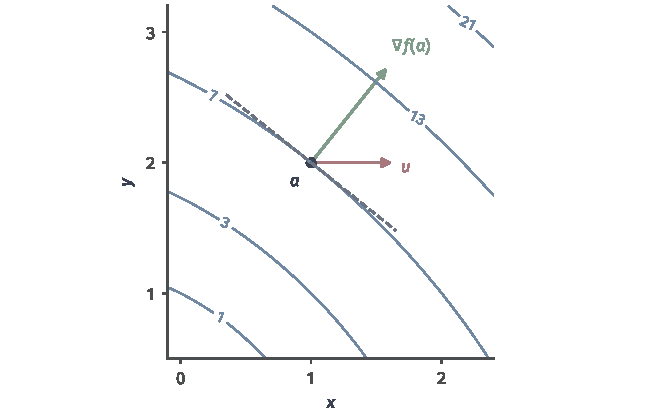
\includegraphics[width=112.0mm]{figures/00-shared/mathematical-preliminaries-upper/00-shared/matplotlib/chapter3-concept-processes/gradient-level-curves.pdf}
 \caption{$f=x^2+xy+y^2$的等值曲线，标注为函数值；基点$a=(1,2)$处$\nabla f=(4,5)^\top$，图中绿箭头按$0.15$倍绘制。灰虚线沿$(5,-4)^\top$，与梯度垂直，因而与经过$a$的等值曲线相切；红箭头为$u=(1,0)^\top$。比较最快上升方向时须先归一化，不能直接比较图中箭头长度。}
 \label{fig:analysis-process-gradient-level-curves}
\end{figure}

\subsection{中值估计与局部Lipschitz性}
\label{sec:multivariable-scalar-mean-value-lipschitz}

微分描述一点附近的变化。要估计两点之间的有限变化，可以沿连接两点的线段把函数限制为一元函数，再使用一元中值定理。前提是整条线段都在定义域内。
记$[\bm x,\bm y]=\{\bm x+t(\bm y-\bm x):0\leq t\leq1\}$为连接两点的线段。
\begin{theorem}[多元标量函数的中值公式]
\label{thm:multivariable-scalar-mean-value}
设$f$在包含$[\bm x,\bm y]$的开集上可微，$\bm x\neq\bm y$。则存在$\theta\in(0,1)$使
\[
 f(\bm y)-f(\bm x)=\nabla f(\bm x+\theta(\bm y-\bm x))^\top(\bm y-\bm x).
\]
\end{theorem}
\begin{proof}
令$\phi(t)=f(\bm x+t(\bm y-\bm x))$，$t\in[0,1]$，它是$f$在线段上的一元切片。$\phi'(t)$就是$f$在点$\bm x+t(\bm y-\bm x)$处沿$\bm y-\bm x$的方向导数，所以$\phi'(t)=\nabla f(\bm x+t(\bm y-\bm x))^\top(\bm y-\bm x)$。
对$\phi$在$[0,1]$上使用一元中值定理，$\phi(1)-\phi(0)=\phi'(\theta)$，这就是所述等式。
\end{proof}
等式说明，两点之间的平均变化率等于线段上某一点沿该方向的瞬时变化率。这是一元“平均斜率等于某点切线斜率”的直接推广。
例如$f(x,y)=x^2+y^2$，$\bm x=(0,0)$、$\bm y=(1,1)$，左侧为$2$；右侧为$\nabla f(\theta,\theta)^\top(1,1)^\top=4\theta$，取$\theta=1/2$即相等，中值点恰为线段中点。

\paragraph{局部Lipschitz性}
\phantomsection
\label{def:multivariable-lipschitz}
定义~\ref{def:ls-lipschitz}已经给出Lipschitz连续与局部Lipschitz连续：存在常数$L$，使输出距离不超过输入距离的$L$倍，局部情形允许常数随邻域改变。那里只说明了这种误差控制的含义，本小节的新任务是由导数求出这样的常数。

中值公式把有限增量写成某点梯度与位移的内积；若梯度的长度有统一上界，就能用输入距离的常数倍控制输出变化。以下距离都取欧氏范数。优化中常用这种控制由步长估计函数值的变化。

先看两个不依赖导数就能读出常数的例子。线性函数$f(\bm x)=\bm a^\top\bm x$满足$|f(\bm x)-f(\bm y)|=|\bm a^\top(\bm x-\bm y)|\leq\lVert\bm a\rVert_2\lVert\bm x-\bm y\rVert_2$，Lipschitz常数可取$\lVert\bm a\rVert_2$，它恰是梯度的长度。
欧氏范数$f(\bm x)=\lVert\bm x\rVert_2$由三角不等式满足$|\lVert\bm x\rVert_2-\lVert\bm y\rVert_2|\leq\lVert\bm x-\bm y\rVert_2$，常数为$1$，尽管它在原点不可微。所以Lipschitz连续本身不要求处处可微。

要把梯度界转化为Lipschitz常数，两点之间的线段必须留在定义域内。若集合$D$中任意两点之间的线段都含于$D$，就称$D$为凸集。在凸开集上，梯度长度的统一上界恰好就是Lipschitz常数。
\begin{theorem}[梯度有界与Lipschitz条件]
\label{thm:multivariable-gradient-lipschitz}
设$U\subseteq\mathbb R^d$为凸开集，$f:U\to\mathbb R$可微。则$f$在$U$上以$L$为Lipschitz常数，当且仅当$\lVert\nabla f(\bm x)\rVert_2\leq L$对所有$\bm x\in U$成立。
\end{theorem}
\begin{proof}
若梯度长度不超过$L$，任取$\bm x\neq\bm y$，凸性保证线段$[\bm x,\bm y]\subseteq U$。由中值公式与内积不等式，
\[
 |f(\bm y)-f(\bm x)|=\bigl|\nabla f(\bm\xi)^\top(\bm y-\bm x)\bigr|\leq\lVert\nabla f(\bm\xi)\rVert_2\lVert\bm y-\bm x\rVert_2\leq L\lVert\bm y-\bm x\rVert_2.
\]
反过来，设$f$以$L$为Lipschitz常数。固定$\bm x$，若$\nabla f(\bm x)\neq\bm0$，取单位方向$\bm u=\nabla f(\bm x)/\lVert\nabla f(\bm x)\rVert_2$，则
\[
 \lVert\nabla f(\bm x)\rVert_2=D_{\bm u}f(\bm x)=\lim_{t\downarrow0}\frac{f(\bm x+t\bm u)-f(\bm x)}t\leq\lim_{t\downarrow0}\frac{Lt}t=L.
\]
梯度为零时不等式自然成立。
\end{proof}
几何上，若坡度处处不超过$L$，沿直线走过距离$\rho$，高度最多改变$L\rho$；反过来，Lipschitz常数也限制了每一点最陡方向的坡度。
例如$f(x,y)=\sin x+\cos y$满足$\lVert\nabla f\rVert_2=\sqrt{\cos^2x+\sin^2y}\leq\sqrt2$，所以它在整个平面上以$\sqrt2$为Lipschitz常数。

定理中的凸性不能省略。在不凸的区域上，梯度可以处处很小，函数值却在两个很近的点之间相差很大。
\begin{example}[非凸区域上梯度有界而不Lipschitz]
\label{ex:multivariable-nonconvex-lipschitz-failure}
取去掉负$x$轴的环形区域$D=\{1<\lVert\bm x\rVert_2<2\}\setminus\{(x,0):x<0\}$，令$f(\bm x)$为点$\bm x$的极角，取值于$(-\pi,\pi)$。$f$在$D$上可微，$\lVert\nabla f\rVert_2=1/r<1$，坡度处处小于$1$。
但取负$x$轴两侧的点$(-1.5,\pm\varepsilon)$，两点距离为$2\varepsilon$，极角却分别接近$\pi$与$-\pi$，相差接近$2\pi$。令$\varepsilon\to0$，函数值之差与距离之比无界，所以$f$在$D$上不是Lipschitz函数。
\end{example}

连接这两点的直线段穿过被去掉的负$x$轴，不在$D$内，中值公式无法使用。$D$内连接两点的路径必须绕过原点，长度远大于$2\varepsilon$。可见梯度界只能沿含于定义域的线段转化为函数值之差的界。

局部情形不需要整个定义域凸。若$f\in C^1(U)$，在每个基点附近取一个包含在$U$内的闭球。连续函数$\lVert\nabla f\rVert_2$在这个闭有界集上有界（定理~\ref{thm:multivariable-extreme-value}），因而在同心的开球上也有界。开球是凸开集，由定理~\ref{thm:multivariable-gradient-lipschitz}，$f$在这个开球上Lipschitz连续，所以$f$局部Lipschitz连续。
各点的局部常数不一定有共同上界：$f(x,y)=x^2$连续可微，但$\lVert\nabla f\rVert_2=2|x|$在全平面无界，因而它不是全域Lipschitz函数。

\paragraph{三种控制的强弱}
至此出现了三种关于函数变化的结论，强度各不相同。连续只保证$\bm x\to\bm a$时$f(\bm x)\to f(\bm a)$，不给出趋近的速度。可微给出渐近的线性近似：误差是$o(\lVert\bm h\rVert_2)$，但对一个给定的有限步长，它不说明误差有多大。梯度的统一界则沿含于定义域的线段控制有限距离上的变化，常数明确，却只估计变化的大小，不估计线性预测还差多少。

要估计一阶预测还差多少，需要把后两种结论结合起来，考察导数本身沿线段怎样变化。第~\ref{sec:multivariable-curvature-error}节的Taylor公式用二阶导数描述这种变化；只用一阶导数的余项界，以及误差被放大多少倍的局部条件数，集中在第~\ref{chap:differential-perturbation-analysis}章讨论。
